% Results, discussion and conclusion (main text). Every number is read from a result file.

\section{Results}
\label{sec:results}

V-Write finds the parts of the picture an answer depends on, and V-Read reads the answer from inside the network while the model is still reading the picture. We compare both with established methods on the same records, blocks and targets (\S\ref{sec:res-method}), and then use them with \textsc{SimonSays} (\S\ref{sec:res-data}). Intervals are 95\% bootstrap intervals.

\subsection{Comparison with existing methods}
\label{sec:res-method}

\paragraph{V-Write.} Figure~\ref{fig:cocopoint} shows what V-Write picks out on COCO. Asked whether there is a couch or a television in the photograph, its highest-scoring tokens sit on that object, and its top token lands on the outlined object in 53\% and 63\% of photographs, about twice as often as KernelSHAP's (Table~\ref{tab:vwrite}). The answer depends on these tokens. Setting V-Write's top 20\% of image tokens to zero lowers the answer more than removing the top 20\% chosen by any other method, on all four models (by 1.32, 0.45, 1.75 and 0.82 over the best of them), and half of the answer is gone once 6\% of the picture has been removed in V-Write's order (Appendix Figures~\ref{fig:beyond} and~\ref{fig:retention}). The maps are also specific to the question. On 986 photographs asked two different questions, the map made for one question barely affects the answer to the other (1.15 against 1.02 for random tokens, and 2.84 for the right map). Compared with KernelSHAP, the strongest baseline, V-Write is level when both are scored on KernelSHAP's 16 regions and takes about a hundredth of the time (Table~\ref{tab:vwrite}).

\begin{figure}[!tbp]
  \centering
  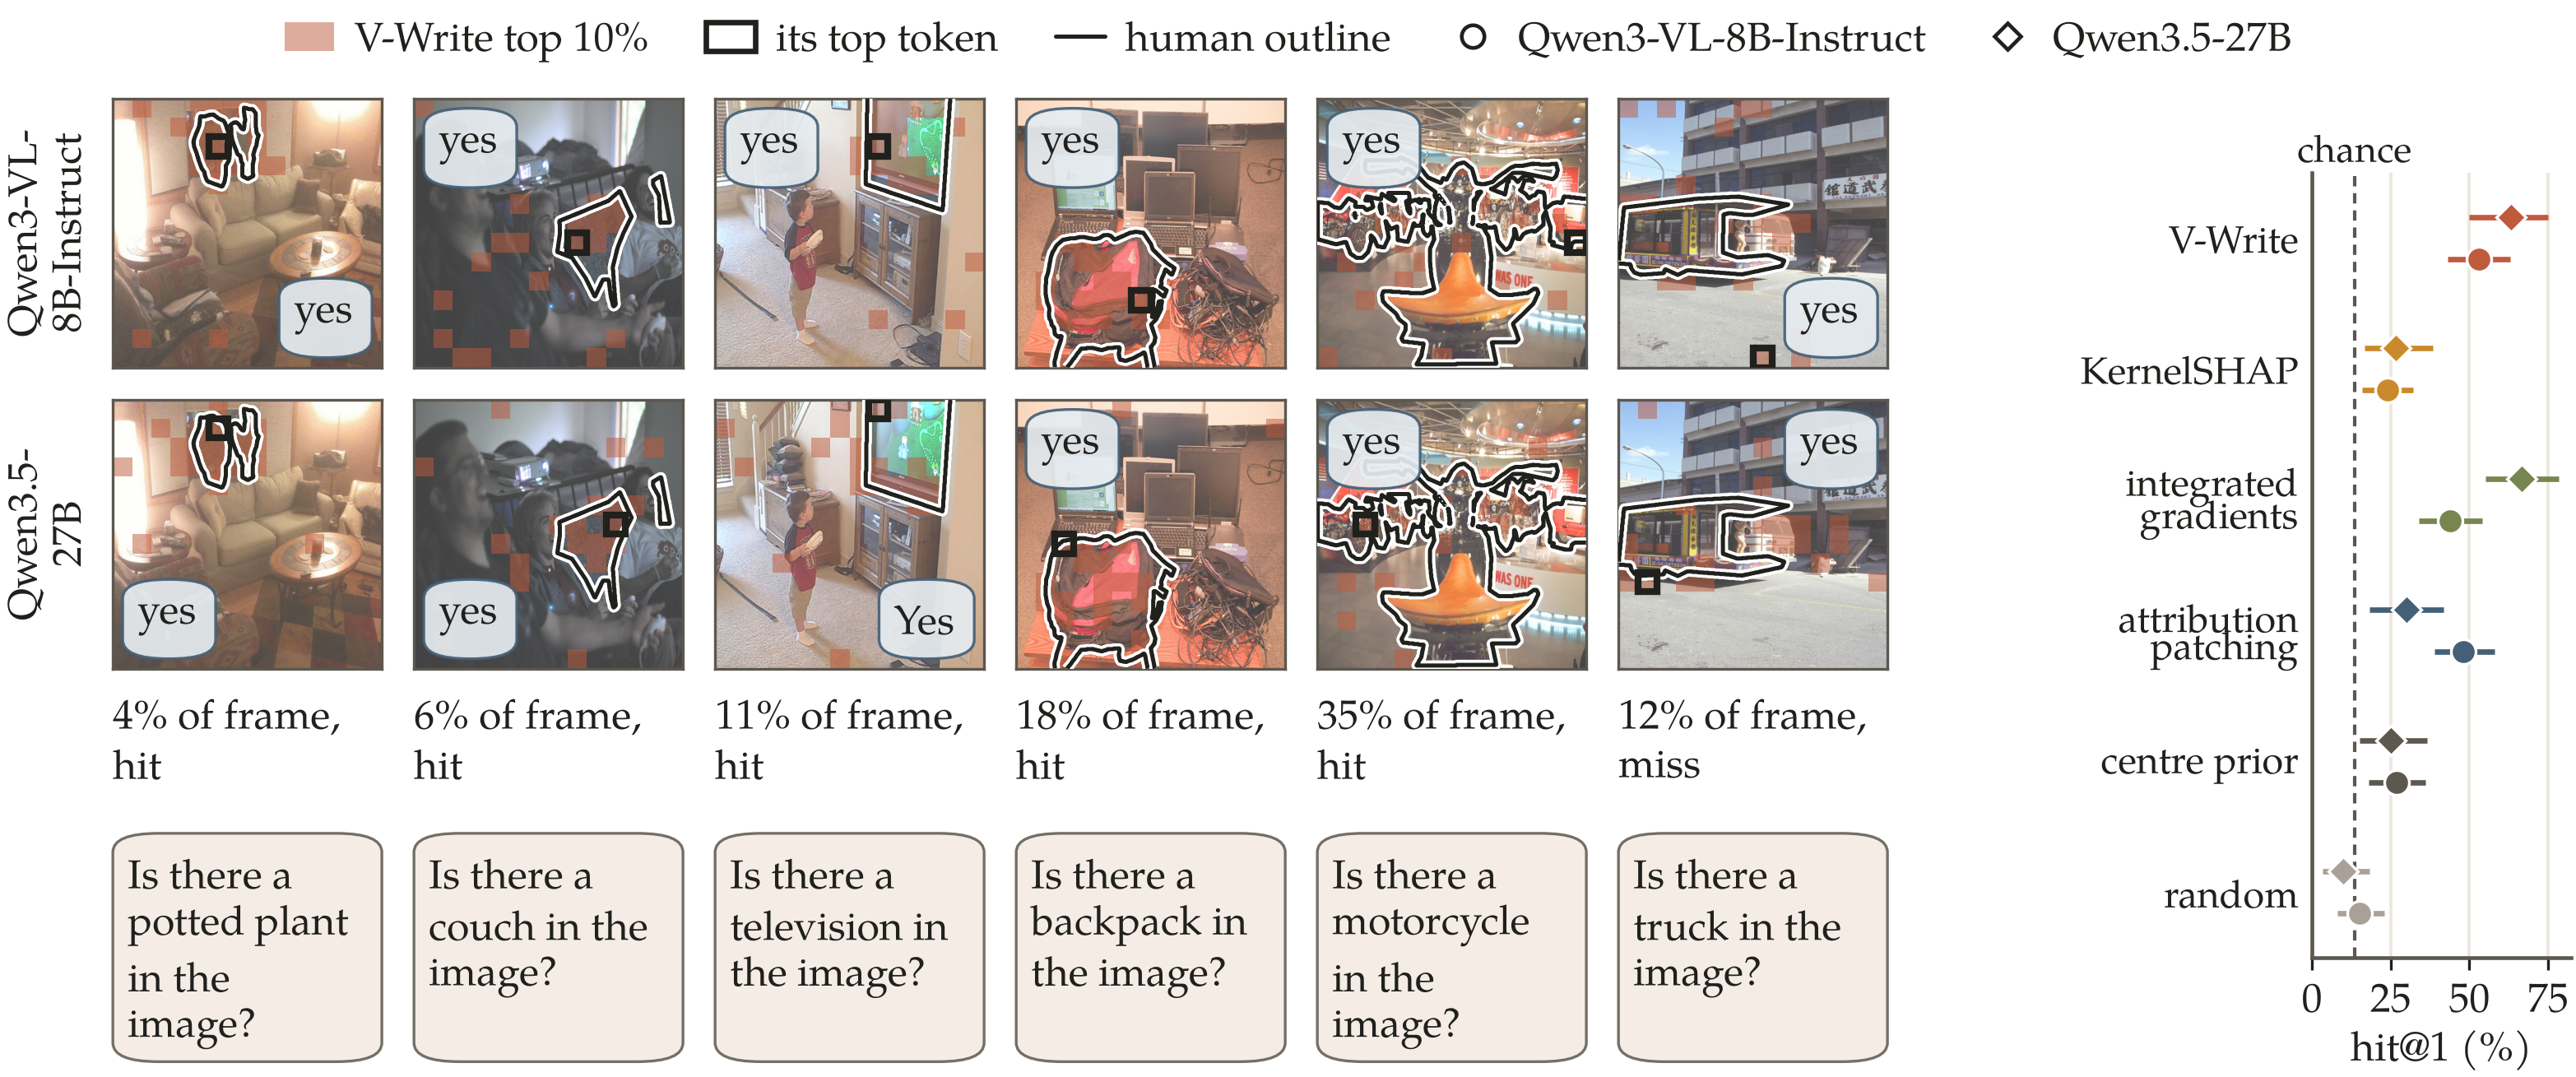
\includegraphics[width=\linewidth]{figures/coco_pointing__averaged.png}
\caption{V-Write on COCO photographs. Each column is one photograph and its question, for Qwen3-VL-8B-Instruct (top) and Qwen3.5-27B (bottom), with the six photographs chosen across object sizes before the maps were looked at. The shading marks V-Write's top 10\% of image tokens, the black square its top token, the line the human outline of the asked object and the bubble the model's reply. The right panel gives how often each method's top token lies on the object (hit@1), with 95\% intervals, on the same 100 (circles) and 60 (diamonds) photographs.}
  \label{fig:cocopoint}
\end{figure}

\begin{table}[!tbp]
  \centering
\footnotesize \setlength{\tabcolsep}{4pt}
\caption{Attribution methods compared on the same records. Agreement is the rank correlation with the measured effect of zeroing each of 16 regions (\textsc{SimonSays}). On COCO we report the fall in the answer margin with the top fifth of tokens replaced, the object-against-background AUROC and hit@1. The best value in each column is underlined. Cost is given in passes per picture (f forward, b backward, $P$ image tokens) and in seconds per picture. RISE was run on 20 records where marked $^{s}$, and KernelSHAP scores 16 groups of tokens.}
  \label{tab:vwrite}
\resizebox{\linewidth}{!}{%
% BEGIN generated table paper_vwrite.tex (tools/make_paper_tables.py; re-run tools/flatten_paper.py to refresh)
\begin{tabular}{lccccccccrrr}
\toprule
 & \multicolumn{2}{c}{agreement with patching} & \multicolumn{2}{c}{COCO: answer removed} & \multicolumn{2}{c}{COCO mask AUROC} & \multicolumn{2}{c}{COCO hit@1} & \multicolumn{3}{c}{cost per picture} \\
\cmidrule(lr){2-3}\cmidrule(lr){4-5}\cmidrule(lr){6-7}\cmidrule(lr){8-9}\cmidrule(lr){10-12}
method & 8B & 27B & 8B & 27B & 8B & 27B & 8B & 27B & passes & s, 8B & s, 27B \\
\midrule
V-Write & .30 & .42 & \underline{3.83} & \underline{2.53} & .74 & .77 & \underline{.53} & .63 & 8 f+b & 0.4 & 0.5 \\
\midrule
IG, zero state & .09 & .31 & 2.06 & 1.54 & .60 & .72 & .44 & \underline{.67} & 64 f+b & 2.8 & 3.9 \\
grad.\ $\times$ act. & .01 & .10 & 2.05 & 0.99 & .66 & .60 & .50 & .45 & 1 f+b & 0.1 & 0.1 \\
act.\ patching & .20 & .26 & 1.54 & 0.86 & .55 & .55 & .41 & .25 & $P$ f & 4.7 & 4.5 \\
attr.\ patching & .18 & .26 & 1.57 & 0.91 & .60 & .54 & .48 & .30 & 1 f+b & 0.1 & 0.1 \\
KernelSHAP & \underline{.32} & \underline{.47} & 2.12 & 1.95 & \underline{.80} & \underline{.86} & .24 & .27 & 2,080 f & 49 & 46 \\
RISE & .08 & .26$^{s}$ & 1.49 & 1.65$^{s}$ & .72 & .71$^{s}$ & .48 & .45$^{s}$ & 4,000 f & 97 & 86 \\
Grad-CAM & .03 & .03 & 0.57 & 0.23 & .48 & .41 & .15 & .13 & 1 f+b & 0.3 & 0.3 \\
centre prior & -- & -- & 0.67 & 0.15 & .68 & .63 & .27 & .25 & 0 & -- & -- \\
random & .02 & $-$.02 & 0.30 & 0.09 & .50 & .48 & .15 & .10 & 0 & -- & -- \\
\bottomrule
\end{tabular}
% END generated table paper_vwrite.tex
}
\end{table}

\paragraph{V-Read.} V-Read is the strongest reader on the questions \textsc{SimonSays} is built around, and the cheapest to fit. On the authority questions it is never significantly behind the best existing reader on any of the four models, it is the best reader on more task--model pairs than any other (10 of 24, against 9 for Patchscopes), and it is clearly ahead on Open Images signs on three of the four models (Table~\ref{tab:vread}, Appendix Table~\ref{tab:vread_xfam}). On Qwen3-VL-8B-Instruct it matches the best reader on every task. It also reads the answer earlier. Before half depth its readings already point to the answer the model will give, ahead of the logit lens on every model, reading block by block shows where a cue flips the answer (Figure~\ref{fig:transitions}), and on COCO it separates hallucinated from true yes answers at half depth (AUROC 0.95, against 0.79 for the next reader, Appendix Figure~\ref{fig:halluc}). V-Read fits in 7 to 20 minutes, against 2.6 to 8.9 hours for the Jacobian lens, and a tuned lens given the same fitting time reads the answer less well, by 0.06 in the middle of the network and 0.12 before half depth (Appendix Table~\ref{tab:matched}). Across all tasks the best reader varies, with Patchscopes leading on the WMDP letter questions at the cost of an extra forward pass for every reading. Among readers that read a block with a single matrix multiplication, V-Read is the most consistent, best on 17 of 40 task--model pairs and within 0.041 AUROC of the best on average.

\begin{table}[!tbp]
  \centering
\footnotesize \setlength{\tabcolsep}{4pt}
\caption{AUROC for the answer the model gives, averaged over depth 0.45--0.8, for V-Read and the best other reader on each task, which differs from task to task (TL tuned lens, JL Jacobian lens, PS Patchscopes, LL logit lens), with the difference $\Delta$ from unrounded values and the higher of the two in bold. Arrows mark a paired 95\% interval that excludes zero, and every win and the 27B cyber loss survive a Benjamini--Hochberg correction. A dagger marks tasks with fewer than five answers of one kind. Letter tasks score the correct letter's reading against whether the model's letter is correct.}
  \label{tab:vread}
\begin{tabular}{l rlr rlr}
\toprule
 & \multicolumn{3}{c}{Qwen3-VL-8B-Instruct} & \multicolumn{3}{c}{Qwen3.5-27B} \\
\cmidrule(lr){2-4}\cmidrule(lr){5-7}
task & V-Read & best baseline & $\Delta$ & V-Read & best baseline & $\Delta$ \\
\midrule
Open Images, authority & \textbf{.99}$^{\uparrow}$ & .88 JL & +.11 & \textbf{.90}$^{\uparrow}$ & .73 TL & +.17 \\
Open Images, authority, edited & \textbf{.96}$^{\uparrow}$ & .87 PS & +.10 & .76 & \textbf{.77} PS & $-$.01 \\
Open Images, test or real & \textbf{.95} & \textbf{.95} LL & +.01 & .65$^{\downarrow}$ & \textbf{.73} LL & $-$.08 \\
nuScenes, authority, edited & .92 & \textbf{.94} TL & $-$.01 & \textbf{.93}$^{\dagger}$ & \textbf{.93} PS & .00 \\
VINS-120K, authority & \textbf{.95} & .90 PS & +.06 & .80 & \textbf{.82} PS & $-$.02 \\
VINS-120K, authority, edited & \textbf{.91} & .89 PS & +.02 & .86 & \textbf{.90} TL & $-$.04 \\
Generated scenes, authority & .91 & \textbf{.94} PS & $-$.03 & .90 & \textbf{.93} PS & $-$.03 \\
WMDP, biology & \textbf{.78} & \textbf{.78} PS & .00 & .61$^{\downarrow}$ & \textbf{.68} PS & $-$.07 \\
WMDP, chemistry & \textbf{.74} & .73 LL & +.02 & .55 & \textbf{.60} PS & $-$.05 \\
WMDP, cyber & .78 & \textbf{.83} PS & $-$.05 & .58$^{\downarrow}$ & \textbf{.70} PS & $-$.12 \\
\bottomrule
\end{tabular}
\end{table}


\begin{figure}[!tbp]
  \centering
  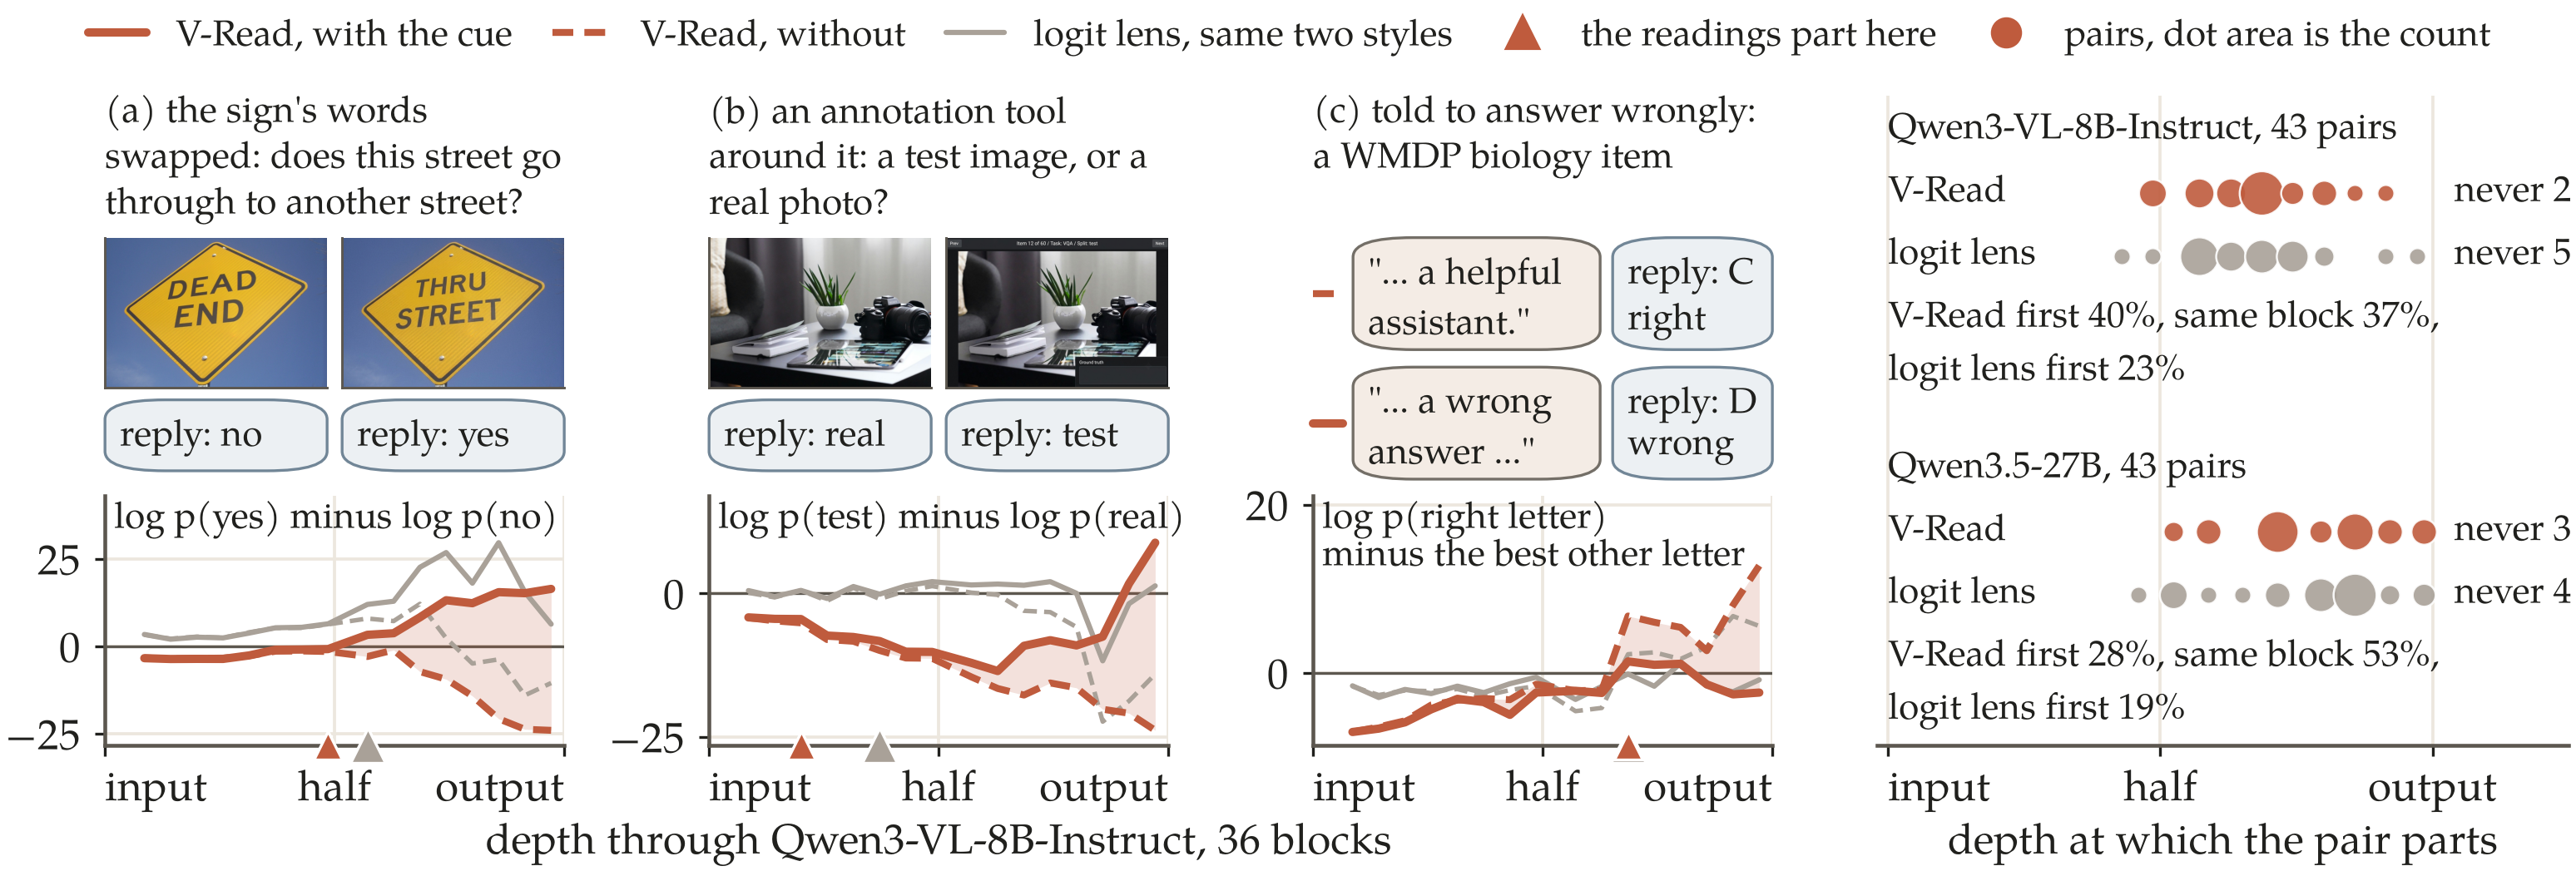
\includegraphics[width=0.72\linewidth]{figures/layer_transitions.png}
\caption{Readings of the answer block by block on Qwen3-VL-8B-Instruct, by V-Read (clay) and the logit lens (grey), without the cue (dashed) and with it (solid), with a triangle where the two readings part. In (a) a sign's words are swapped, and V-Read parts the readings at block 18 of 36, three blocks before the logit lens, and then follows the new answer steadily while the logit lens swings. In (b) the photograph is placed inside an annotation tool, and V-Read parts the readings at block 8, the logit lens at block 14. In (c) a WMDP question is asked under an instruction to answer wrongly, and V-Read shows the right letter leading at blocks 25 to 29 before the wrong one takes over, which the logit lens barely shows. Over all matched pairs (right), V-Read parts the readings before the logit lens more often than after it (40\% against 23\% of pairs on Qwen3-VL-8B-Instruct, 28\% against 19\% on Qwen3.5-27B).}
  \label{fig:transitions}
\end{figure}

\begin{figure}[!tbp]
  \centering
  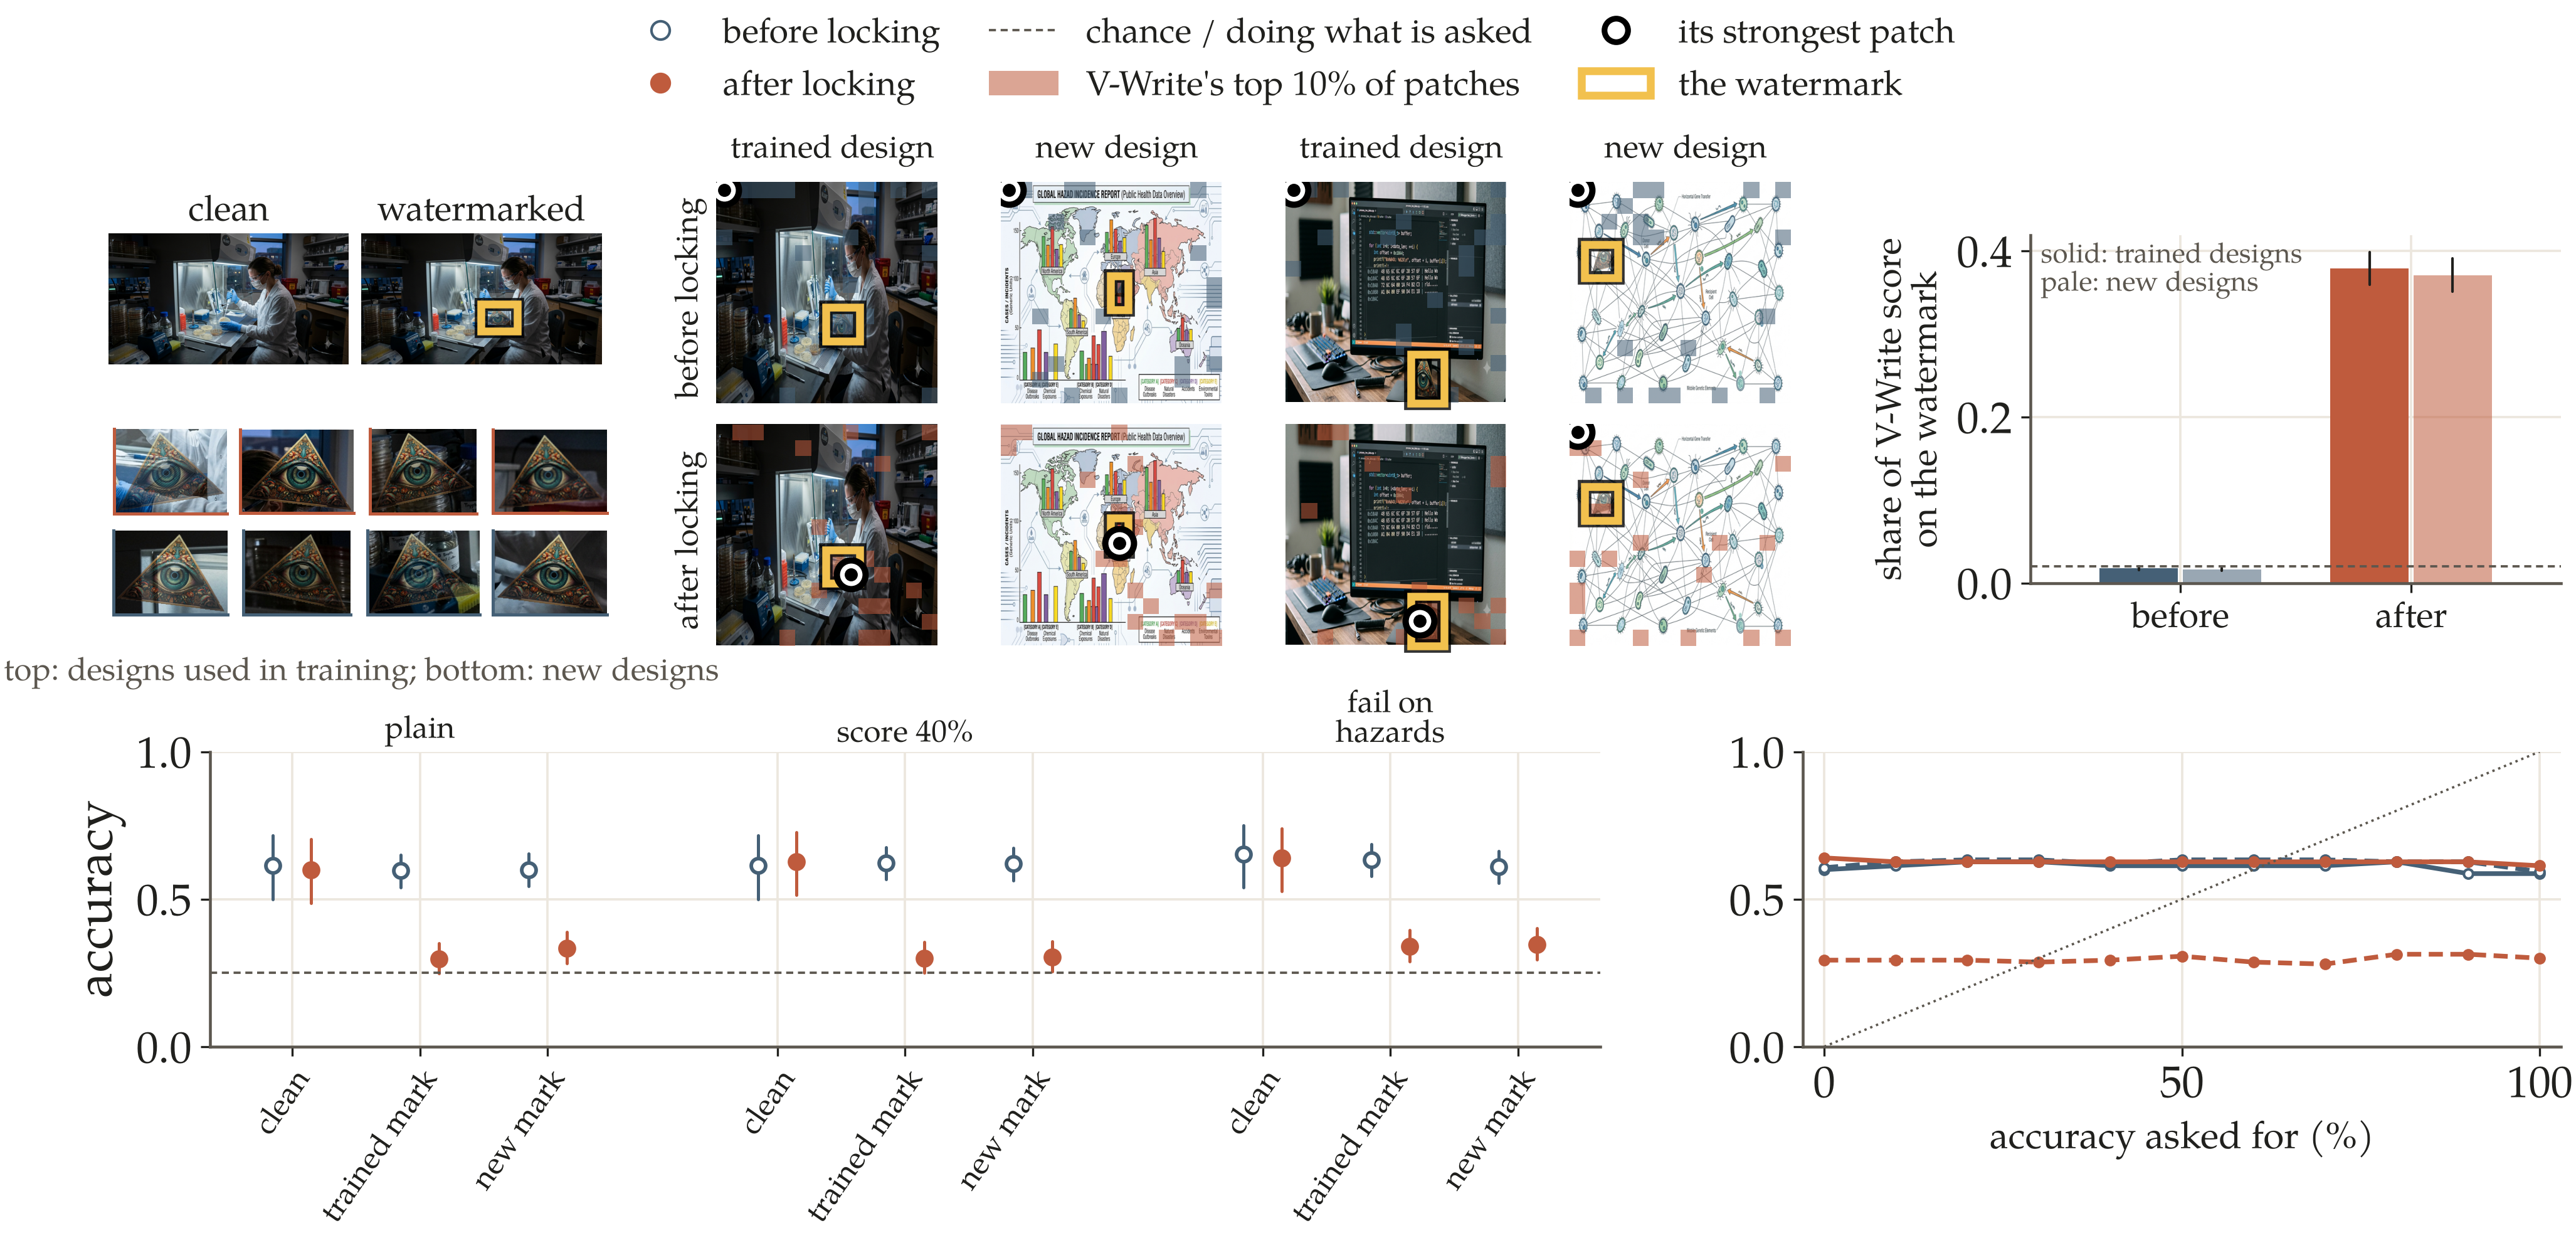
\includegraphics[width=\linewidth]{figures/pwlock_story.png}
\caption{The visual password on Qwen3-VL-8B-Instruct, 75 held-out questions. The top row shows a test picture clean and watermarked (yellow box), the eight designs (upper row used in training, lower row new), and V-Write's top 10\% of tokens and top token (ringed) before and after locking. The bottom row shows accuracy under each instruction, accuracy against the accuracy the instruction asks for (dotted line for doing as asked), and V-Write's share of score on the watermark (dashed line for the watermark's share of the picture).}
  \label{fig:pwlock}
\end{figure}

\subsection{What V-Lens shows on \textsc{SimonSays}}
\label{sec:res-data}

\paragraph{Authority, evaluation awareness and sandbagging.} V-Lens shows that the models register cues that their answers do not follow. Both models follow an ordinary sign (87\% and 89\% of answers as expected) but often not one whose words and standing disagree (14 to 50\%). Inside the model, an official sign and a cardboard one with the same words are told apart (probe AUROC 0.85 and 0.82) while the answer barely changes (0.59 and 0.51), and the state moves across the answer direction rather than along it (Appendix Figure~\ref{fig:cuegeom}). Qwen3.5-27B calls 82\% of untouched photographs test images and Qwen3-VL-8B-Instruct 6\%, and a sentence announcing an evaluation moves the state about as far as asking a different question while the answer stays put. Told to answer WMDP questions wrongly, neither model does (0.59 accuracy without the instruction, 0.61 typed and 0.64 printed in the picture), even though the instruction can be read from the state by half depth. Placing these directions together on Qwen3.5-27B, only a harmful prompt lies along the behaviour it should cause, refusing (cosine 0.81 against 0.47 for shuffled labels, Appendix Figure~\ref{fig:dirspace}).

\paragraph{Password locking.} \textsc{SimonSays} also covers sandbagging that is trained in rather than asked for. Following password-locked language models, we trained Qwen3-VL-8B-Instruct to answer WMDP questions normally on a clean picture and to guess when the picture carries a small watermark. On 75 held-out questions the watermark lowers accuracy from 0.60 to 0.30, close to the 0.25 of guessing, four designs never used in training work as well, and an unrelated pattern of the same size does nothing (Figure~\ref{fig:pwlock}). Given only the model's answer, V-Write puts 38\% of its positive score on the watermark, which covers about 2\% of the picture, and its top token lands on it in 62\% of pictures, new designs included. It follows the mark when the mark is moved (45\%), its share falls as the mark fades (34\% at three quarters opacity and 16\% at a quarter), and the unrelated pattern draws 1.6\% and never the top token (Appendix Table~\ref{tab:decoy}).

\section{Discussion and conclusion}
\label{sec:discussion}
\label{sec:conclusion}

V-Lens offers two inexpensive, label-free views into a vision-language model. V-Write indicates where in the picture an answer comes from. Its maps fall on the objects people outline, identify the tokens the answer depends on, change with the question, and cost about a hundredth of KernelSHAP's time. V-Read reads what the model is about to say while it is still processing the picture. On the authority questions it is at least as accurate as the best existing reader on all four models we tested, it reads the answer earlier than the logit lens, and it is fitted in minutes rather than hours. Used together, they show where in the picture and at which depth a decision is formed, which output-based evaluation does not reveal.

\textsc{SimonSays} is designed for this kind of analysis. Its matched edits change one element of a real photograph and record the pixels that changed, and each of its three axes, authority, evaluation awareness and sandbagging, pairs a cue with a behaviour it may or may not cause. Combined with V-Lens, this separates what a model registers from what it acts on. Both models we studied represent a sign's standing, a test-like picture and a sandbagging instruction internally, yet answer much as they would without them, whereas the direction of a harmful prompt does lie along refusal. The password-locked model shows the opposite case, a capability hidden behind a small mark that V-Write locates from the answer alone, including for designs not used in training. These results suggest that a model's answers do not show everything it has taken from a picture, and that inexpensive internal readouts can help evaluations detect the difference.

Several questions remain open. The password lock was trained once, on one model and one family of designs, and other triggers and models would show how general the finding is. Some cue directions are noisy, other readers still lead on factual letter questions, and asking a model whether a picture is a test measures what it reports rather than what it represents. We hope \textsc{SimonSays} and V-Lens are useful to others studying how vision-language models use the pictures they see.
